\documentclass[oneside,twocolumn]{article}

\usepackage{sectsty}
\allsectionsfont{\bfseries\sffamily} % <---- omitting \bfseries still gives bold font
\renewcommand*{\familydefault}{\sfdefault}
\setlength{\parindent}{0in}
\usepackage{amsmath}
\usepackage{graphicx}
\usepackage{color}
%\usepackage{verbatim}
%\usepackage{url}

\definecolor{copper}{RGB}{175,102,53}

\begin{document}

% Skip an extra line between paragraphs
\addtolength{\parskip}{\baselineskip}

\section*{\color{copper} \huge How BECCA works}

\textsc{Becca} 0.6.0 

Brandon Rohrer, December 2014

\textsc{Becca}'s long term goals are captured in its name: brain-emulating cognition and control architecture. This is a detailed description of the architecture and the algorithms that underlie it. It is a summary of the python code. If any discrepancies exist, the code is the authoritative source. This description omits some of the details of implementation and computational bookkeeping that aren't essential to understanding its principles of operation.  

\textsc{Becca} belongs to a class of machine learning algorithms called reinforcement learners. The distinguishing characteristic of a reinforcement learning agent is that it receives an explicit reward signal, which it tries to maximize. (Figure~\ref{rl}) 

\begin{figure}[ht]
\centering
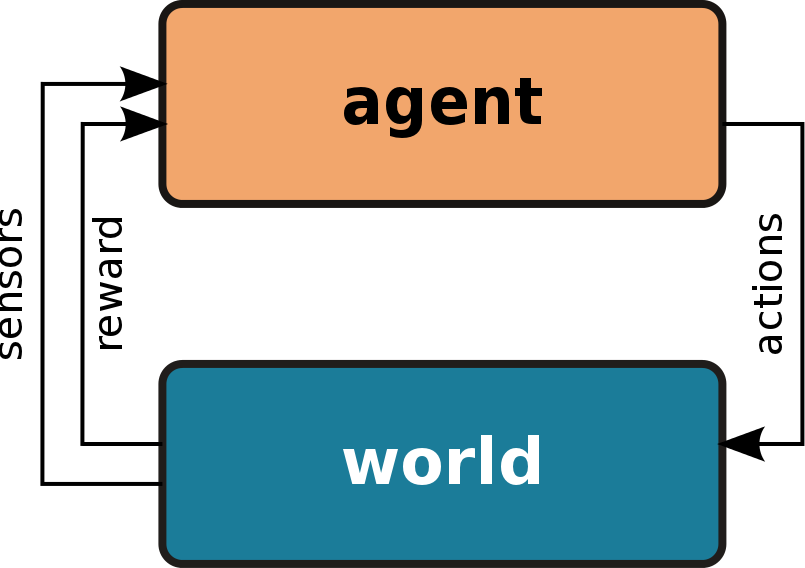
\includegraphics[height=5.0cm]{figs/rl.png}
\caption{A reinforcement learning agent.}
\label{rl}
\end{figure}

To be more precise, \textsc{Becca} consists of both an unsupervised learning algorithm that extracts features from the data, and a reinforcement learning algorithm that learns which sequences of features tend to result in positive outcomes. (Figure~\ref{learners})

\begin{figure}[ht]
\centering
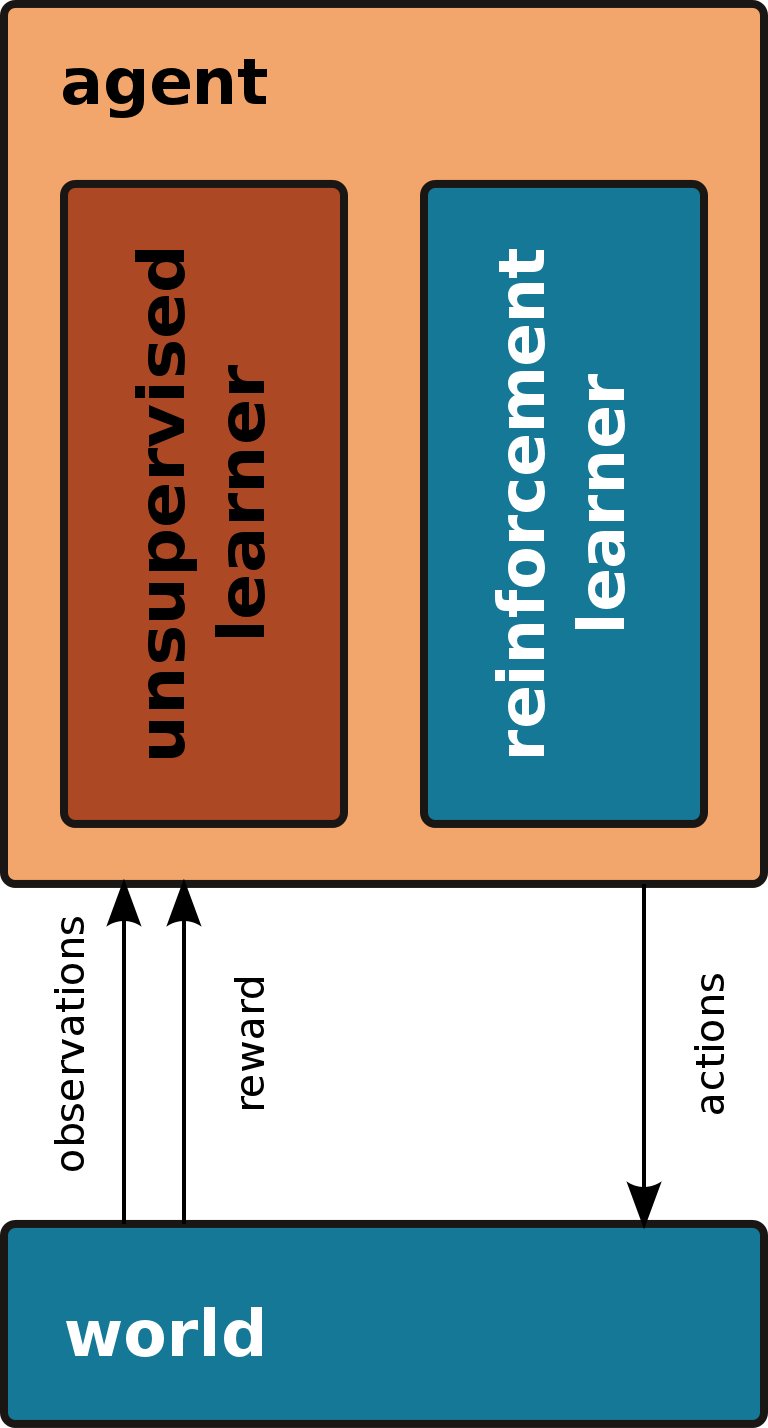
\includegraphics[height=10.0cm]{figs/learners.png}
\caption{\textsc{Becca}'s agent contains both an unsupervised feature extractor and a reinforcement learner.}
\label{learners}
\end{figure}

\textsc{Becca} is designed so that it doesn't know (or need to know) anything about the world it's operating in. This is so that it can be used as the learning portion of any embodied agent, a general purpose robot brain.

\section*{\color{copper} AGENT}

The agent is, in essence, the brain. Everything else---the hardware, the sensors, and the rest of the universe---is included in the world. In fact, any system-specific pre-processing of sensor inputs and post-processing of actions are part of the world. The agent handles only sensor and reward inputs and produces action outputs. It does this in discrete time steps.  

\begin{figure}[ht]
\centering
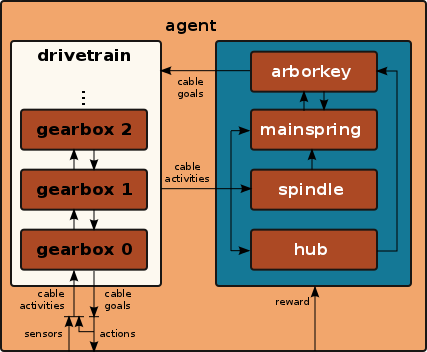
\includegraphics[height=6.0cm]{figs/agent.png}
\caption{The agent consists of a hierarchy of gearboxes, arranged to form the drivetrain (the unsupervised learner), all of which are connected to a central complex of consisting of the hub, spindle, mainspring, and arborkey (the reinforcement learner).}
\label{agent}
\end{figure}

The agent contains one or more gearboxes in a hierarchical arrangement. A central collection of elements--the hub, spindle, mainspring, and arborkey--is connected to them all. (Figure~\ref{agent}) The gearboxes build the sensory information into spatio-temporal features whose complexity and extent grows greater in each subsequent level. The first gearbox takes an array of cable activities as inputs at each time step, which are composed of the latest sensor activities, and a copy of the actions from the previous time step. Here, cables are a physical metaphor for channels or lines that carry a signal. Cable activities are the set of signal values on an array of cables at one point in time. Each gearbox takes a set of cable activities as inputs and produces a set of cable activities as outputs. They are cascaded, such that the cable activity outputs of one gearbox are also the inputs to the next.

At each time step, the cable activities are propagated upward through the entire drivetrain. Then, copies of the cable activity inputs to each gearbox are sent to the hub, spindle, and mainspring. The hub uses cable activities together with the reward to select a hub cable goal for one of the gearboxes. The spindle chooses one cable to attend to. The mainspring uses the attended cable and reward as a basis for constructing short term and long term memory and for learning delayed rewards. The arborkey evaluates potential goals from the hub with the help of the mainspring and periodically issues one of those goals back to the drivetrain. This centrally-selected goal is analogous to deliberate behavior in humans. The gearboxes then propagate this goal downward through the drivetrain, together with any internal goals (similar to reactions or auto-pilot behavior in humans) that they generate. A subset of the cable goals that emerge from the lowest gearbox correspond to an array of actions. These are passed back to the world. They are they only decisions or influence that the agent has on the world around it.

\section*{\color{copper} GEARBOX}

Gearboxes are core structural elements of the architecture and naturally form a hierarchy, the drivetrain, in which each is supported by the one below. Each gearbox contains some cogs and a ziptie, a cable-clustering element. (Figure~\ref{gearbox}) 

\begin{figure}[ht]
\centering
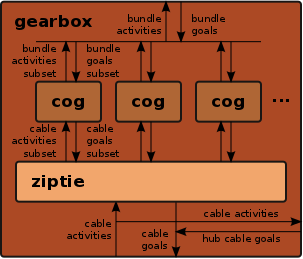
\includegraphics[height=6.0cm]{figs/gearbox.png}
\caption{Each gearbox consists of a ziptie cable clusterer and a number of cogs, all operating in parallel.}
\label{gearbox}
\end{figure}

The gearbox takes a set of cable activities as inputs. The ziptie organizes them into groups over time and assigns each group of cables to a single cog. Cogs are where cable activities are combined together across cables and over time to build spatio-temporal features. They take arrays of cable activities as inputs and combine those into bundles. Their outputs are the activities in each of those bundles. The bundle activities of all the cogs are combined together into a single array to form the output of the gearbox.

The cable activities are normalized such that they fall on an interval from zero (the lowest cable activity ever experienced on that cable) to one (the highest). This helps keep every bock  insensitive to the range of cable activities it takes in, including sensor values from the world.

The number of gearboxes in the drivetrain grows as higher-level features are created. Once the number of bundles created collectively by all the cogs in gearbox $n$ exceeds a fraction threshold of the gearbox's total capacity (.5), then gearbox $n+1$ is created automatically. This allows the feature hierarchy to adaptively scale to represent arbitrary complexity in the data being observed. 

\section*{\color{copper} COG}

Like their mechanical counterparts, cogs are relatively simple devices whose true value is realized when they are used in parallel with a number of their fellows. Each cog consists of a daisychain and a ziptie. (Figure~\ref{cog}) 

\begin{figure}[ht]
\centering
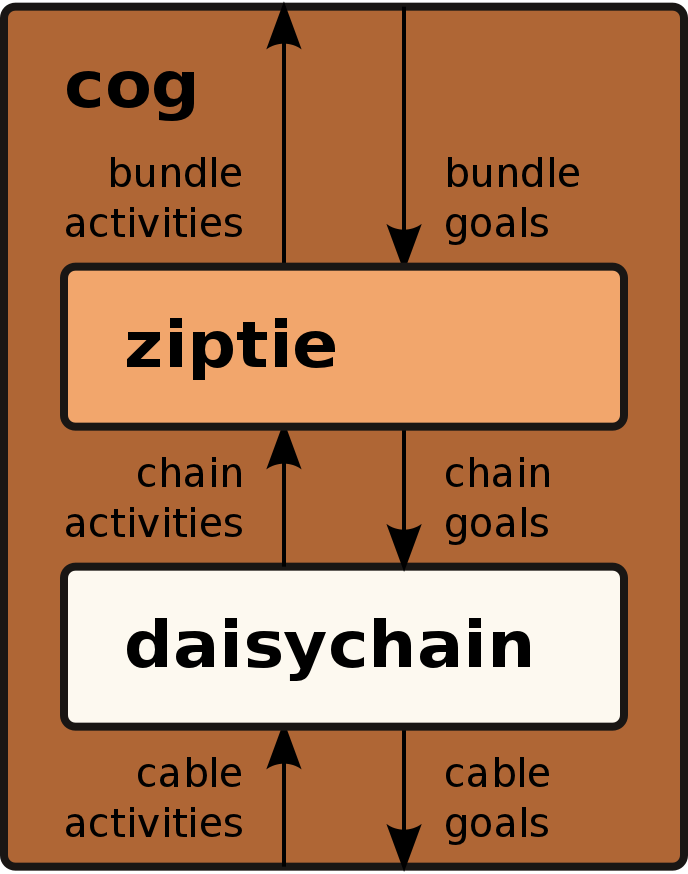
\includegraphics[height=7.0cm]{figs/cog.png}
\caption{Each cog contains a daisychain and a ziptie.}
\label{cog}
\end{figure}

The daisychain identifies the relative prevalence of all possible cable activity sequences from one time step to the next, i.e. chains. The ziptie clusters commonly co-occurring chains into bundles. A bundle of chains is a pattern of signals that covers multiple cables and multiple time steps. Another way of expressing this is to say that is has both spatial and temporal extent or is a spatio-temporal pattern. The bundles that the cog generates are data-driven features. Taken in aggregate, all the bundles from all the cogs form a feature set that \textsc{Becca} can use to represent its relationship to its world and to choose its future actions. 

\section*{\color{copper} ZIPTIE}

Ziptie is a clustering algorithm used throughout \textsc{Becca}. In contrast to many unsupervised learning algorithms which cluster individual data points, ziptie clusters signals or time series of data points or dimensions in many-dimensional input stream. This is analogous to bundling groups of cables with zipties. Like all algorithms in \textsc{Becca}, it is incremental, performing its functions iteratively at each time step. Ziptie identifies cables whose activities tend to be high at the same time. Although at any given moment the cable activities may be very different, over time they will tend to be co-active. 

The ziptie updates and maintains a map from cables to bundles. (Figure~\ref{ziptie}) This map dictates how cable activities are translated into bundle activities and how bundle goals are translated into cable goals. 

\begin{figure}[ht]
\centering
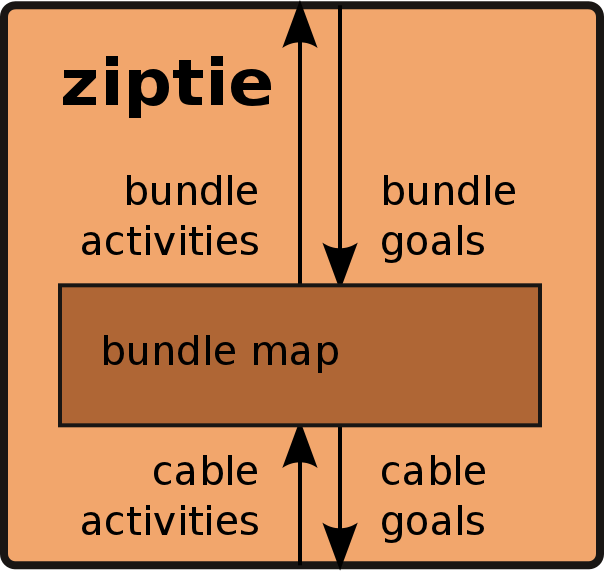
\includegraphics[height=4.0cm]{figs/ziptie.png}
\caption{A ziptie clusters its cables together into bundles.}
\label{ziptie}
\end{figure}

The ziptie groups cables into bundles based on how often the cables' activity levels tend to be simultaneously high. Any cable can be a member of one bundle, many bundles, or no bundles. Membership is binary (all or nothing), but there is no reason the algorithm couldn't be extended to represent partial membership.

\section*{\color{copper} Bundle activity}

Bundle activity is a weighted combination of its constituent cable activities. Some inhibition occurs between bundles that share cables. Initial bundle activities are calculated by taking the generalized mean of the cable activities with a negative exponent.  
The generalized mean, $M_p$, is given by:

\begin{equation*}
M_p(x) = {\frac{1}{n}\left( \sum_{i=1}^{n}x_i^p  \right)}^{\frac{1}{p}} 
\end{equation*}

For $p = 1$, $M_p$ is the arithmetic mean. For $\lim_{p \to 0}$ it is the geometric mean. For $\lim_{p \to \infty}$ it gives the maximum value. And for   $\lim_{p \to -\infty}$ it gives the minimum. A negative exponent weights the lower cable activities more heavily. 

Ziptie makes a first pass at each bundle's activity .

\begin{eqnarray*}
a &=& M_m(c)\\ 
a &:& \mbox{initial bundle activity}\\ 
c &:& \mbox{activities of cables in the bundle}\\
m &:& \mbox{generalized mean exponent} = -4
\end{eqnarray*}

If a cable contributes to multiple bundles, the activity it contributes to each will be somewhat inhibited.

\begin{eqnarray*}
d &=& c \left( \frac{a}{b} \right) ^ k\\ 
a &:& \mbox{initial bundle activity}\\ 
b &:& \mbox{highest initial bundle activity}\\ 
c &:& \mbox{original cable activity}\\
d &:& \mbox{inhibited cable activity}\\
k &:& \mbox{inhibition exponent} = 6
\end{eqnarray*}

The final bundle activity is calculated in the same way as the initial bundle activity, except that it uses the inhibited cable activities. A single cable ends up contributing different activation levels to the different bundles of which it's a member.

A cable can also have a residual non-bundle activity, signifying that it has signal energy that has not been applied to activating any bundle.

\begin{eqnarray*}
f &=& \max \left (0, c - \sum d \right)\\ 
c &:& \mbox{original cable activity}\\
d &:& \mbox{inhibited cable activity for each bundle}\\
f &:& \mbox{non-bundle activity}
\end{eqnarray*}

\section*{\color{copper} Bundle nucleation}

Non-bundle cable activity is accumulated over time. If it accumulates to a high enough level, that signals the ziptie that a new bundle needs to be created.

\begin{eqnarray*}
g &=& g + (f  (1 - g)  - c  g  p )  q\\ 
f &:& \mbox{non-bundle activity}\\
g &:& \mbox{nucleation energy}\\
c &:& \mbox{cable activity}\\
p &:& \mbox{energy decay rate} = .01\\
q &:& \mbox{nucleation energy rate} = .0001
\end{eqnarray*}

A cable's nucleation energy exceeds a threshold (.05),  then it nucleates a new bundle, that is, it becomes the sole member of a new bundle.
          
\section*{\color{copper} Bundle agglomeration}

Bundles accumulate agglomeration energy from cables whose non-bundle activity is correlated with their own. 

\begin{eqnarray*}
h &=& fa\\ 
h &:& \mbox{co-activity}\\
f &:& \mbox{non-bundle activity}\\
a &:& \mbox{bundle activity}\\
\end{eqnarray*}

Each cable's non-bundle activity is distributed to agglomeration energy with each bundle proportionally to their co-activities.

\begin{eqnarray*}
s &=& s + f  \frac{a}{\sum a} (h (1-s) - c s p) t\\ 
s &:& \mbox{agglomeration energy between}\\
&& \mbox{a cable and a bundle}\\
f &:& \mbox{non-bundle activity}\\
a &:& \mbox{bundle activity}\\
\sum a &:& \mbox{sum of all bundle activities}\\
h &:& \mbox{co-activity}\\
c &:& \mbox{cable activity}\\
p &:& \mbox{energy decay rate} = .01\\
t &:& \mbox{agglomeration energy rate} = .01\\
\end{eqnarray*}
                                      
When the agglomeration energy exceeds a threshold (.05), the cable is added to the bundle.

\section*{\color{copper} Cable goals}
        
Bundle goals are translated back into cable goals as they propagate down the drivetrain of gearboxes. For each cable, the goals for the bundles it contributes to are summed in such a way that the magnitude of the sum is never greater than one.

\begin{eqnarray*}
u &=& S(v)\\ 
u &:& \mbox{cable goal}\\
v &:& \mbox{bundle goals}
\end{eqnarray*}

The bounded sum function, $S$, never produces a total greater than one, given that its arguments are all less than one.

\begin{eqnarray*}
S(x) & = & A \left (\sum B(x) \right ) \\
A(x) & = & 1 - \frac{1}{x + 1} \\ 
B(x) & = & \frac{x}{1 - x} - 1 \\
A&:& \mbox{maps the interval} [0, \infty)\\
&& \mbox{onto the interval} [0, 1) \\
B&:& \mbox{maps the interval} [0, 1)\\
&& \mbox{onto the interval} [0,\infty ) \\
\end{eqnarray*}


\section*{\color{copper} DAISYCHAIN}

Dasiychain is an incremental algorithm that estimates the probability of one cable being active following another. It represents this as a conditional probability: given that one cable is active what is the expected activity of a second cable in the next time step. (Figure ~\ref{daisychain}) High expected chain activities indicate sequences of cable activities that co-occur regularly. They identify temporal structure in the data. 

Expected chain activities are similar to transition probabilities in Markov models. The difference is that in a Markov model, only one state can be occupied at each time step. This is analogous to just one cable being active. In a daisychain, many cables can be completely or partially active at once. As a result, transition probabilities can sum to much more than one. 

\begin{figure}[ht]
\centering
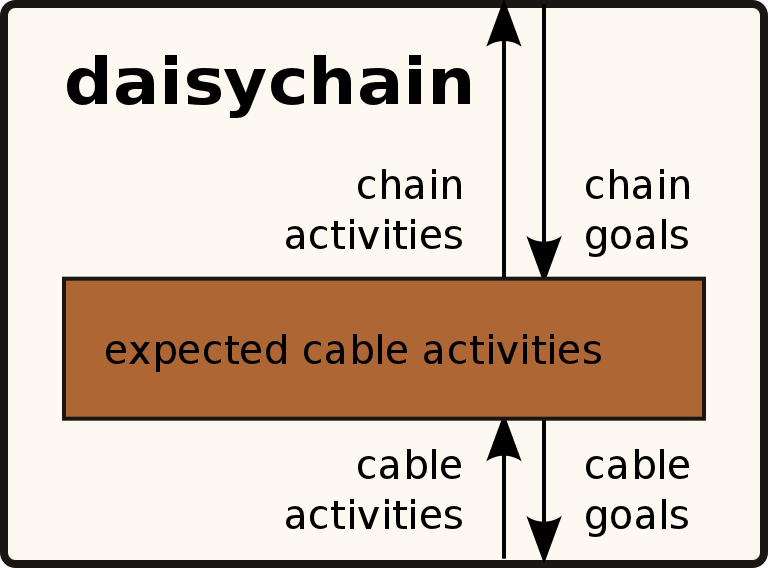
\includegraphics[height=4.0cm]{figs/daisychain.png}
\caption{A daisychain identifies commonly occurring cable sequences, or chains.}
\label{daisychain}
\end{figure}

\section*{\color{copper} Expected chain activity}

A temporal sequence of one cable being active, followed by another, is a chain. The activity of a chain is given by the product of the two cable activities involved.

\begin{eqnarray*}
c &= & ab\\ 
c &:& \mbox{chain activity} \\
a &:& \mbox{cable activity} \\
b &:& \mbox{another cable activity,}\\
&& \mbox{from the previous time step}\\
\end{eqnarray*}

A leaky accumulation of the activity on each cable and on each chain is also maintained.

\begin{eqnarray*}
d &= & d + c - \frac{1}{df}\\ 
d &:& \mbox{accumulated chain activity} \\
c &:& \mbox{chain activity} \\
f &:& \mbox{aging time constant} = 10^6 \\
\end{eqnarray*}

\begin{eqnarray*}
g &= & g + b - \frac{1}{gk}\\ 
g &:& \mbox{accumulated cable activity} \\
b &:& \mbox{previous cable activity} \\
k &:& \mbox{chain update rate} = .1 \\
\end{eqnarray*}

The expected chain activities are maintained and updated based on the current chain activities. 

\begin{eqnarray*}
h &= & h + (c-h)b \left ( \frac{1 - k}{g} + k \right)\\ 
h &:& \mbox{expected chain activities} \\
c &:& \mbox{chain activity} \\
b &:& \mbox{previous cable activity} \\
k &:& \mbox{chain update rate} = .1 \\
g &:& \mbox{accumulated cable activity} \\
\end{eqnarray*}

\section*{\color{copper} Expected chain activity deviation}

In addition, the expected {\em deviation} from the expected chain activities are maintained and updated based on the difference between the current and expected chain activities. 

\begin{eqnarray*}
m &= & m + (|c-h|-m) b \left ( \frac{1 - k}{g} + k \right)\\ 
m &:& \mbox{expected chain activity deviation} \\
c &:& \mbox{chain activity} \\
h &:& \mbox{expected chain activities} \\
b &:& \mbox{previous cable activity} \\
k &:& \mbox{chain update rate} = .1 \\
g &:& \mbox{accumulated cable activity}
\end{eqnarray*}

\section*{\color{copper} Predictions}

The temporal structure captured in the expected chain activities provide a basis for making short-term predictions.The reaction is the predicted next set of cable activities. 

\begin{eqnarray*}
n &= & \frac{\sum h a}{\sum{a}} \\
n &:& \mbox{predicted cable activity} \\
h &:& \mbox{all expected chain activities that include} \\
&& \mbox{the cable activity being predicted} \\
a &:& \mbox{current cable activities}
\end{eqnarray*}

The most recently observed cable activities can be compared to those that would have been predicted from the previous cable activities to find surprising events.

\begin{eqnarray*}
p &= &  \frac{\sum \frac{a | a - n |}{m}}{\sum{\frac{a}{m}}} \\
p &:& \mbox{surprise} \\
a &:& \mbox{current cable activities} \\
n &:& \mbox{predicted cable activity, based on} \\
&& \mbox{previous cable activity} \\
m &:& \mbox{expected chain activity deviation} 
\end{eqnarray*}

\section*{\color{copper} Cable goals}

As chain goals are propagated down through the daisychain, they are combined to form the cable goals. Each cable goal is a weighted, bounded sum of all the goals of the chains it belongs to.

\begin{eqnarray*}
s &= &  S(qa + n) \\
s &:& \mbox{cable goal} \\
S &:& \mbox{bounded sum operator} \\
q &:& \mbox{chain goals} \\
a &:& \mbox{current cable activities} \\
n &:& \mbox{predicted cable activity} \\
\end{eqnarray*}

\section*{\color{copper} HUB}

The hub is where reinforcement learning is implemented and decisions are made. It takes in copies of all gearboxes' input cable activities, as well as the reward. It maintains an estimate of expected reward for every cable activity-cable goal sequence, or chain, similar to the daisychain's estimate of future cable activity for every cable activity chain within a gearbox. 

The reward signal is normalized such that it falls on an interval from zero (the lowest reward ever experienced) to one (the highest). This way, \textsc{Becca} is insensitive to the range of reward values covered by the world. The chains that consistently result in higher reward are identified and exploited. 
 
The hub gathers cable activities from the drivetrain. Using the current set of cable activities, it chooses a cable goal at each time step. It then associates changes in reward with each activity-goal pair. This is where the hub differs from daisychain. The transition chains in daisychain are from cable activity to next cable activity, rather than from cable activity to next cable goal. Like daisychain, the hub does this incrementally, adjusting the estimate by a small amount each time. It also creates a running sum of each chain's activity history, which slowly decays over time. This calculation is very similar to the one used in daisychain.

\begin{eqnarray*}
c &= & ab\\ 
c &:& \mbox{chain activity} \\
a &:& \mbox{cable activity} \\
b &:& \mbox{cable goal magnitude}\\
\end{eqnarray*}

\section*{\color{copper} Reward estimation}

In order to associate transitions with delayed rewards, a reward trace is calculated. It is a summation of reward, decayed over time.

\begin{eqnarray*}
q &= & \sum_{t=0}^m \frac{p_t}{t+1}\\ 
q &:& \mbox{full reward trace} \\
t &:& \mbox{time steps into the future} \\
m &:& \mbox{trace length} = 10\\
p &:& \mbox{current reward}\\
p_t &:& \mbox{reward $t$ time steps}\\
&& \mbox{into the future}\\
\end{eqnarray*}

The expected reward trace associated with each chain is updated using the instantaneous and cumulative chain activities.

\begin{eqnarray*}
r &= & r + (q - r)c k \\ 
r &:& \mbox{expected reward trace} \\
q &:& \mbox{observed reward trace} \\
c &:& \mbox{chain activity} \\
k &:& \mbox{reward learning rate} = .1 \\
\end{eqnarray*}

\section*{\color{copper} Optimism-driven exploration}

\textsc{Becca} is mildly optimistic. It assumes that any goal it hasn't pursued is likely to have some small reward. The lowest reward an agent has ever encountered is assigned a value of 0 and the highest is assigned a value of 1. Untried goals are assumed to have a value of .5. This motivates \textsc{Becca} to try goals that it hasn't tried before, until it learns that they aren't worth repeating.

\section*{\color{copper} Hub goal selection}

The estimated reward value for all the chains is weighted by the square of current cable activities. The winning cable goal is the one with the highest weighted average value. The hub passes that goal to the arborkey. 

\begin{eqnarray*}
w &= & \mbox{argmax} \frac {\sum rc^2}{\sum c^2}\\ 
w &:& \mbox{goal cable} \\
r &:& \mbox{estimated reward value at this time step} \\
c &:& \mbox{cable activity} \\
\end{eqnarray*}

Of course the final goal selection is performed by the arborkey. Whenever the arborkey selects a goal, it is passed back to the hub so that the estimated rewards can be updated appropriately 

\section*{\color{copper} SPINDLE}

The spindle selects a single cable activity to attend to. It picks the one with the highest activity, weighted by how long it has been since it was last attended.

\begin{eqnarray*}
s &= & \left( 1 - \frac {1}{t} \right) c \\ 
a &= & \mbox{argmax } s \\ 
s &:& \mbox{salience} \\
a &:& \mbox{attended cable} \\
t &:& \mbox{time steps since attended} \\
c &:& \mbox{cable activity} \\
\end{eqnarray*}

Intuitively, very intensely active cables are given the strongest preference. Very recently attended cables are suppressed avoid neglecting them.

The spindle handles attention and salience. It has a huge impact on the behavior of the agent. As it stands, it's simplistic, only taking into account cable activity and how recently it was observed. There are a lot of other aspects of attention that experimental psychologists have identified. I hope that I'll get to incorporate these into future versions of \textsc{Becca}.

\section*{\color{copper} MAINSPRING}

The mainspring learns the expected reward associated with cable-goal chains in a manner very similar to that of the hub. However, it learns rewards that occur on a longer timescale. This allows the agent to learn complex and delayed relationships.

The mainspring also learns expected cable saliences based on previously attended cables.

Rather than learning on all currently active cables, the mainspring learns on recently attended cables. The set of recently attended cables is analogous to short term memory in human psychology. Recently attended cable are decayed hyperbolically. That means that their original salience when attended is multiplied by a $1/t$ term. The least energetic cable is dropped from the set at each time step.

\begin{eqnarray*}
d &= & \frac {s}{t} \\ 
d &:& \mbox{decayed salience} \\
s &:& \mbox{original salience} \\
t &:& \mbox{time steps since attended} \\
\end{eqnarray*}

The reward trace is calculated exactly as in the hub. The estimated reward for each chain is then estimated as in the hub.


\begin{eqnarray*}
c &= & a^2 b\\ 
c &:& \mbox{chain activity} \\
a &:& \mbox{decayed salience} \\
b &:& \mbox{cable goal magnitude}\\
\end{eqnarray*}

\begin{eqnarray*}
r &= & r + (q - r)c k \\ 
r &:& \mbox{expected reward trace} \\
q &:& \mbox{observed reward trace} \\
c &:& \mbox{chain activity} \\
k &:& \mbox{reward learning rate} = .1 \\
\end{eqnarray*}

\begin{eqnarray*}
s &= & \frac {\sum rd}{\sum d}\\ 
s &:& \mbox{overall estimated reward value} \\
r &:& \mbox{estimated reward value by cable} \\
d &:& \mbox{decayed salience} \\
\end{eqnarray*}

This is a way to evaluate potential goals over longer time scales than the hub can alone.

\section*{\color{copper} ARBORKEY}

The function of the the arborkey is to make the final decision about which goals to issue and when. The hub passes its best goal candidate to the arborkey at each time step. The arborkey reevaluates it using the mainspring's longer term reward estimate. Then the arborkey notes the goal, its expected reward, and when it was put forward as a candidate.

A decayed expected reward is calculated for each goal in the candidate list. The expected reward is a function of the expected reward and how recently they were observed. 

\begin{eqnarray*}
d &=& \frac {r}{1 + wt}\\
d &:& \mbox{decayed expected reward} \\
r &:& \mbox{expected reward value} \\
w &:& \mbox{reward decay rate} = .5 \\
t &:& \mbox{time steps since the candidate was put forward}\\
\end{eqnarray*}

A restlessness term is added to the decayed expected rewards to calculate the goal values. If the highest goal value is higher than reward currently being experienced, it is chosen as the goal and executed. When this happens, the list of goal candidates is wiped clean and the process begins again. 


\begin{eqnarray*}
v &=& d + yt\\
v &:& \mbox{goal value} \\
d &:& \mbox{decayed expected reward} \\
y &:& \mbox{action propensity} = .16 \\
t &:& \mbox{time steps since a goal was executed}\\
\end{eqnarray*}

If the list of goal candidates grows to be more than 25 candidates long, the candidate with the lowest decayed expected reward is dropped from the list.  

 

\section*{\color{copper} SUMMARY}

One of the agent's greatest strengths is that it doesn't start off knowing or believing anything about the world it's connected to. There are only three arrows that connect the two: the sensors and reward flowing in and the actions flowing out. It was designed this way so that \textsc{Becca} could be used for a brain in a robot of any type, physical or virtual, localized or distributed, commercial or experimental, rigid or flexible, mobile or fixed, walking, rolling, or articulated. For that matter it can be used to learn and control any system that has sensors and can take commands: stock trading, HVAC, retail shipping and receiving, or a self-driving  automobile.


%\begin{figure}[ht]
%\centering
%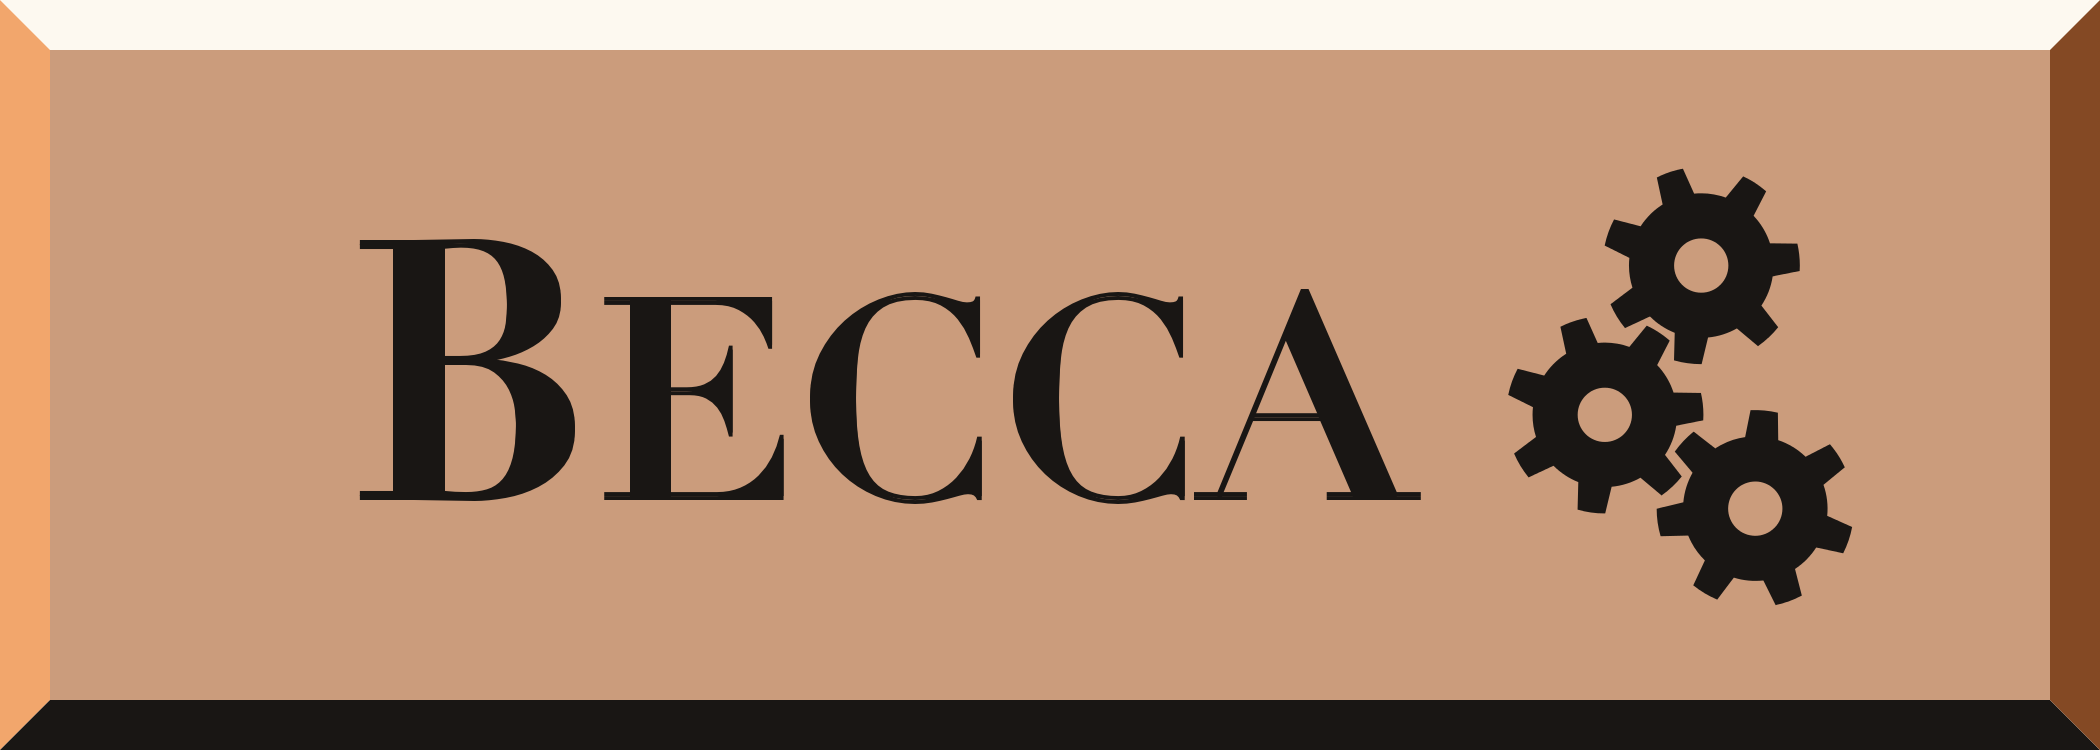
\includegraphics[height=1.5cm]{figs/logo_plate.png}
%\end{figure}


%\bibliographystyle{plain}
%\bibliography{master}
\end{document}
